\documentclass{beamer}
%\usetheme{Ilmenau}
%\usecolortheme{beaver}

\usepackage[slovak,american]{babel}
\usepackage[utf8]{inputenc}
\usepackage{graphicx}
\usepackage{adjustbox}

 \usepackage{xcolor}
 
 \newsavebox\MBox
\newcommand\Cline[2][red]{{\sbox\MBox{$#2$}%
  \rlap{\usebox\MBox}\color{#1}\rule[-2.2\dp\MBox]{\wd\MBox}{1pt}}}

%\usefonttheme{serif}

%\definecolor{UKOrange}{HTML}{ef9424} %
\definecolor{UKOrange}{HTML}{7a2c18} %
\definecolor{UKBrown}{HTML}{a96d5e} %
\definecolor{UKLight}{HTML}{d8b6ab} %
\definecolor{UKDark}{HTML}{7a4f44}
\definecolor{UKDarker}{HTML}{4d312b} 
\definecolor{UKDarkest}{HTML}{2e1e1a}
\definecolor{UKRed}{HTML}{bf1f1c}

\setbeamertemplate{footline}[frame number]{}
\setbeamertemplate{navigation symbols}{}

%\usecolortheme{beaver}
\setbeamertemplate{itemize item}[square]
\setbeamercolor{itemize item}{fg = UKBrown}
\setbeamercolor{itemize subitem}{fg = UKLight}
\setbeamercolor{enumerate item}{fg = UKDark}

\setbeamercolor{footnote}{fg=UKLight}
\setbeamercolor{footnote mark}{fg=UKLight}
\setbeamerfont{footnote}{size=\tiny}
\renewcommand\footnoterule{}

\usetheme{default}
\beamertemplatenavigationsymbolsempty
\setbeamercolor{title}{fg=white, bg=UKBrown}
\setbeamercolor{frametitle}{fg=white, bg=UKBrown}
\setbeamercolor{block title}{bg=UKBrown, fg= white}
\setbeamercolor{block body}{bg =UKLight, fg = UKDarkest}

\setbeamercolor{block title alerted}{bg=UKOrange, fg= white}
\setbeamercolor{block body alerted}{bg =UKLight, fg = UKDarkest}


%\setbeamercolor{section in toc}{fg = UKBrown}
%\setbeamercolor{section in toc}{fg = UKDarkest}

% odstrani gulicky
\renewcommand*{\slideentry}[6]{}

\useoutertheme[subsection=false]{miniframes}
\AtBeginSection[]{\subsection{}}

\setbeamercolor{below lower separation line head}{bg=UKDark}
\addtobeamertemplate{headline}{}{%
  \begin{beamercolorbox}[colsep=0.5pt]{below lower separation line head}
  \end{beamercolorbox}
}
%\setbeamercolor*{mini frame}{fg=white,bg=UKRosy}
\setbeamercolor{section in head/foot}{fg=UKLight, bg=UKDark}

\usepackage{etoolbox}
\makeatletter
\preto{\@verbatim}{\topsep=0pt \partopsep=0pt }
\makeatother

%\setbeamertemplate{itemize/enumerate body begin}{\normalsize}
%\setbeamertemplate{itemize/enumerate subbody begin}{\normalsize}




%\newcommand{\codeblock}[2]{ \begin{block}{#1} \begin{verbatim}#2\end{verbatim}\end{block}}

%\defbeamertemplate*{title page}{customized}[1][]
%{
%  \begin{centering}
%    \begin{beamercolorbox}[sep=8pt,center]{title}
%      \usebeamerfont{title}\inserttitle
%    \end{beamercolorbox}
%  \end{centering}
%  \bigskip
%
%\begin{columns}[onlytextwidth,T]
%
%
%  \column{27mm}
%  \includegraphics[width=27mm]{images/logoFMFI.png}
%  
%  \column{\dimexpr\linewidth-54mm-6mm}
%  \centering
%  \vspace{5mm}  
%  \usebeamerfont{author}\insertauthor\par
%  \vspace{5mm}
%  \usebeamerfont{institute}\insertinstitute\par
%
%  \column{27mm}
%  \includegraphics[width=27mm]{images/logoUK.png}  
%\end{columns}
%\centering
%\vspace{7mm}
%  \usebeamerfont{date}\insertdate\par
%}

\DeclareMathOperator*{\argmin}{arg\,min}
\newcommand{\e}[1]{$\cdot 10^{#1}$}
\newcommand*\mean[1]{\bar{#1}}

\newcommand*{\Z}{\mathbb{Z}}

%\newcommand{\codeblock}[2]{ \begin{block}{#1} \begin{verbatim}#2\end{verbatim}\end{block}}




\title[7. cvičenie]{Advanced Image Processing - Morphology}
\author[Kocur]{Ing. Viktor Kocur \\{\small viktor.kocur@fmph.uniba.sk}}
\institute{DAI FMFI UK}
\date{6.11.2018}

\begin{document}
\selectlanguage{american}

\begin{frame}
  \titlepage
\end{frame}

\section{Morphological operations}
\subsection{Erosion and Dilation}

\begin{frame}
\frametitle{Definition}
  \begin{block}{Definition - binary image}
  Let $E \subseteq \Z^d$ be a grid and $A$ is its subset, then this subset is a binary image.
  \end{block}
  
  \begin{block}{Definition - structural element}
  Structural element $B$ is also a binary image, e.g. $B \subseteq E$. It can also be moved which we denote as  $B_z = \{b + z | b \in B\}$ for $\forall z \in E$.
  \end{block}

  \begin{block}{Definition - erosion}
  Erosion $A \ominus B = \{z \in E | B_z \subseteq A \}.$
  \end{block}
  
  \begin{block}{Definition - dilation}
  Dilation $A \oplus B = \bigcup_{a \in A} B_a$
  \end{block}
\end{frame}

\begin{frame}
\frametitle{Intuitive explanation} 
\noindent\makebox[\textwidth]{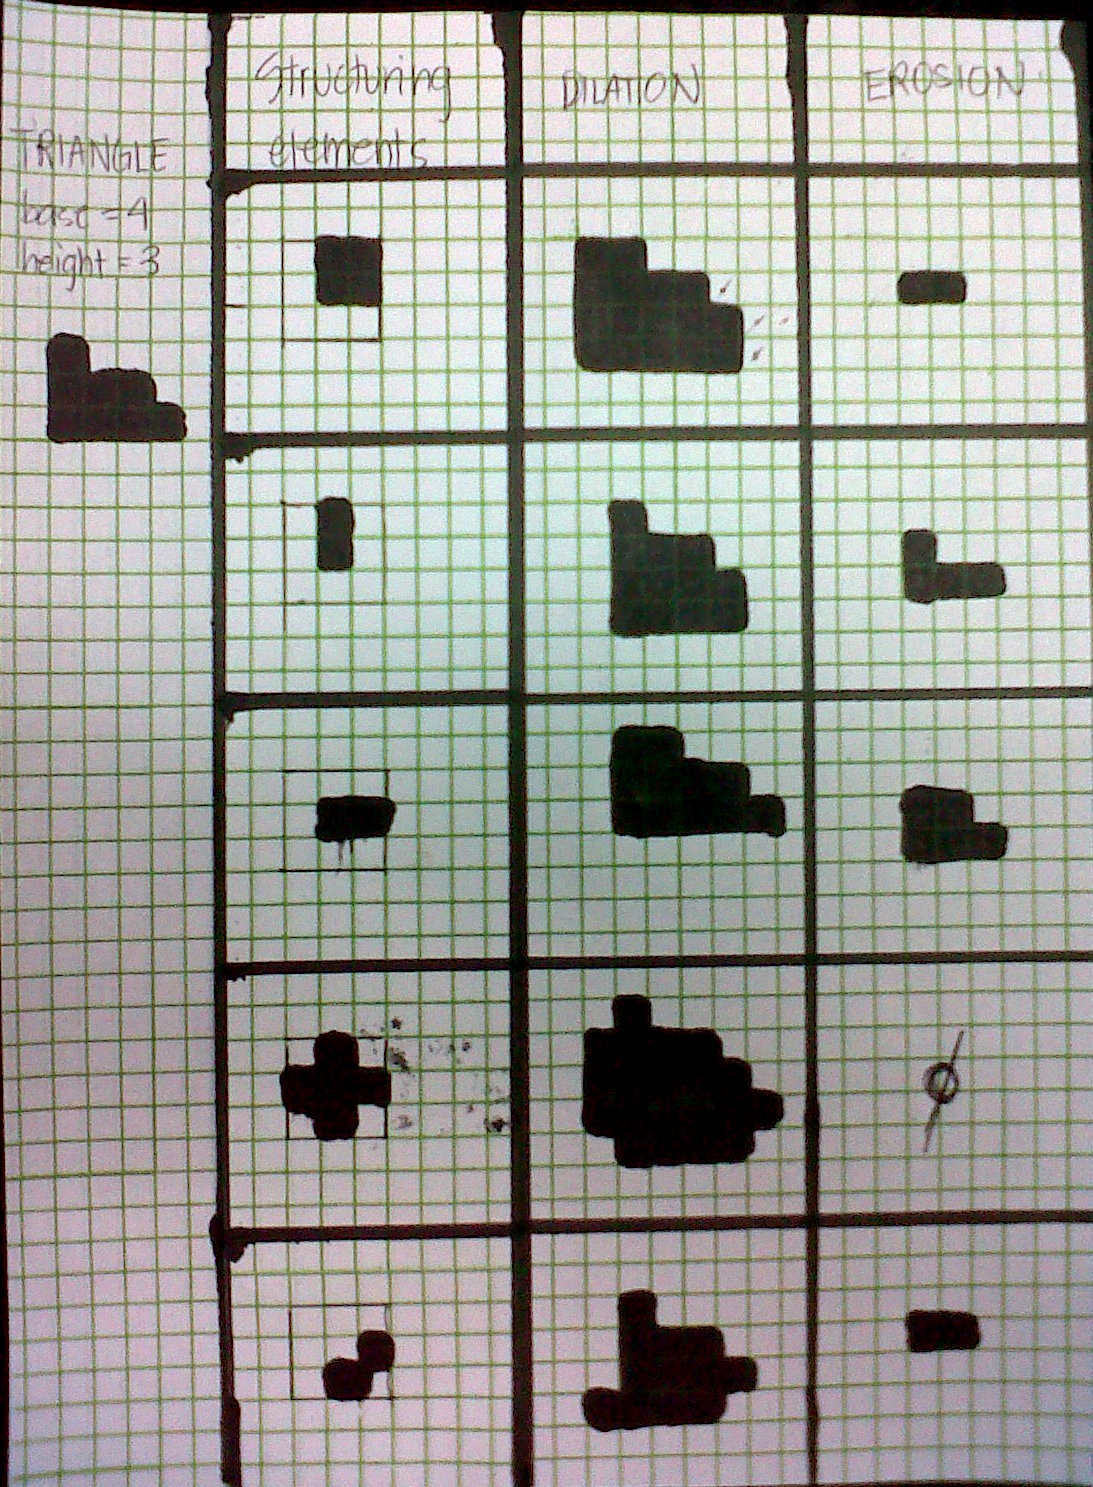
\includegraphics[width=0.5\linewidth]{triangle.jpg}}
\end{frame}


\begin{frame}
\frametitle{Matlab} 
  \begin{block}{strel}  
  SE = strel(name, params) - returns structural element with given parameters. Names are 'diamond', 'disk', 'line', 'octagon', 'rectangle' a 'square'.
  \end{block}
    
  \begin{block}{imerode}
  imerode(I,SE) - returns erosion of image I with structural element SE. Works also for grayscale, but we will leave that for the next week.
  \end{block}
  
    \begin{block}{imdilate}
  imdilate(I,SE) - returns dilation of image I with structural element SE. Works also for grayscale, but we will leave that for the next week.
  \end{block}
  
  \begin{block}{Exercise}
  Test out dilation and erosion on the image jeden.jpg with various SE.
  \end{block}
\end{frame}

\begin{frame}
\frametitle{Properties}
  \begin{block}{Commutativity}
  $A \oplus B = B \oplus A$ 
  \end{block}
    
  \begin{block}{Associativity}
  $A \oplus (B \oplus C) = (A \oplus B) \oplus C$ 
  \end{block}
  
  \begin{block}{Shift invariance}
  $A \oplus B_z = (A \oplus B)_z$
  \end{block}
  
  \begin{block}{Duality}
  Erosion and dilation are mutually dual. E.g. erosion of the image is the same as dilation if the inverse image and vice versa.
  \end{block}
\end{frame}


\subsection{Opening and closing}

\begin{frame}
\frametitle{Definitions}
  \begin{block}{Definition - closing}
  Closing A with structural element B is  $(A \oplus B) \ominus B$. Closing usually fills holes in the binary image.
  \end{block}
  
  \begin{block}{Definition - opening}
  Opening A with structural element B is $(A \ominus B) \oplus B$. Opening usually removes smaller objects such as noise from image.
  \end{block}
\end{frame}

\begin{frame}
\frametitle{Matlab - opening and closing}
  \begin{block}{imopen}
  imclose(I, SE) - returns closing of image I with structural element SE
  \end{block}
  
  \begin{block}{imopen}
  imopen(I, SE) - returns opening of image I with structural element SE
  \end{block}  
  
  \begin{block}{regionprops}
  s = regionprops(BW, 'Centroid') - returns a struct containing field Centroi which contains the centers of individual objects in the binary image.
  \end{block} 
\end{frame}

\begin{frame}
\frametitle{Exercises}
  \begin{block}{Exercise}
  Use morpholigal operations to count the circles in image connected.png and lines\_and\_circles.png.
  \end{block}  
  
  \begin{block}{Exercise}
  Use adaptive thresholding, filtration and morphological operations to count the large circles in Kruhy.jpg.
  \end{block}  
  
  \begin{block}{Exercise}
  Use morphological operations to remove the artefacts from the image fingerprint.png.
  \end{block}
  
  \begin{block}{Exercise}
  Use morphological operations to find holes in the fence in the image fence.png.
  \end{block}
\end{frame}


\subsection{Edges}

\begin{frame}
\frametitle{Edges}
  \begin{block}{Edge detection}
  We can use morphological operations to find edges of objects. For a binary image $I$ we can find edges if we one of the logical rules $I \neq I \ominus SE$, $I \neq I \oplus SE$, or $I \ominus SE \neq I \oplus SE$.
  \end{block}    
  
  \begin{block}{Exercise}
  Find edges in the image motyle.png. Try to use different SEs.
  \end{block}    
\end{frame}

\subsection{Hit-miss}
\begin{frame}
\frametitle{Hit-miss}
  \begin{block}{Hit-miss}
  Hit-miss transforms the image using two structural elements so that  $HM = I \ominus SE_1 \cap (E / I) \ominus SE_2$. In other words only those pixels remain where $SE_1$ 'fits' a $SE_2$ doesn't.
  \end{block}    
  
  \begin{block}{bwhitmiss}
  bwhitmiss(BW, SE1, SE2) - returns hit-miss according to the definition
  \end{block}   
  
  \begin{block}{bwhitmiss}
  bwhitmiss(BW, interval) - Same as bwhitmiss(BW, interval == 1, interval == -1)
  \end{block}   
  
  \begin{block}{Exercise}
  Find corners in boxes.png using Hit-miss.
  \end{block}   
  
   
\end{frame}


\end{document}